%
% Wirbelschleppe.tex -- Erleutert Wirbelschleppen
%
% !TEX root = ../../buch.tex
% !TEX encoding = UTF-8
%
\section{Wirbelschleppe}
Da wir nun ein grundsätzliches Verständnis haben, kommen wir nun zu einer praktischen Anwendung, den Wirbelschleppen.
An einem nebligen Tag kann man sie an einem Flughafen gut beobachten. 
Aber wieso entstehen sie eigentlich? 
Wo genau starten sie und wo ist deren Ende?
Wieso schaudert es Kleinflugzeug-Piloten, wenn sie diesen Begriff hören?
\begin{figure}
\centering
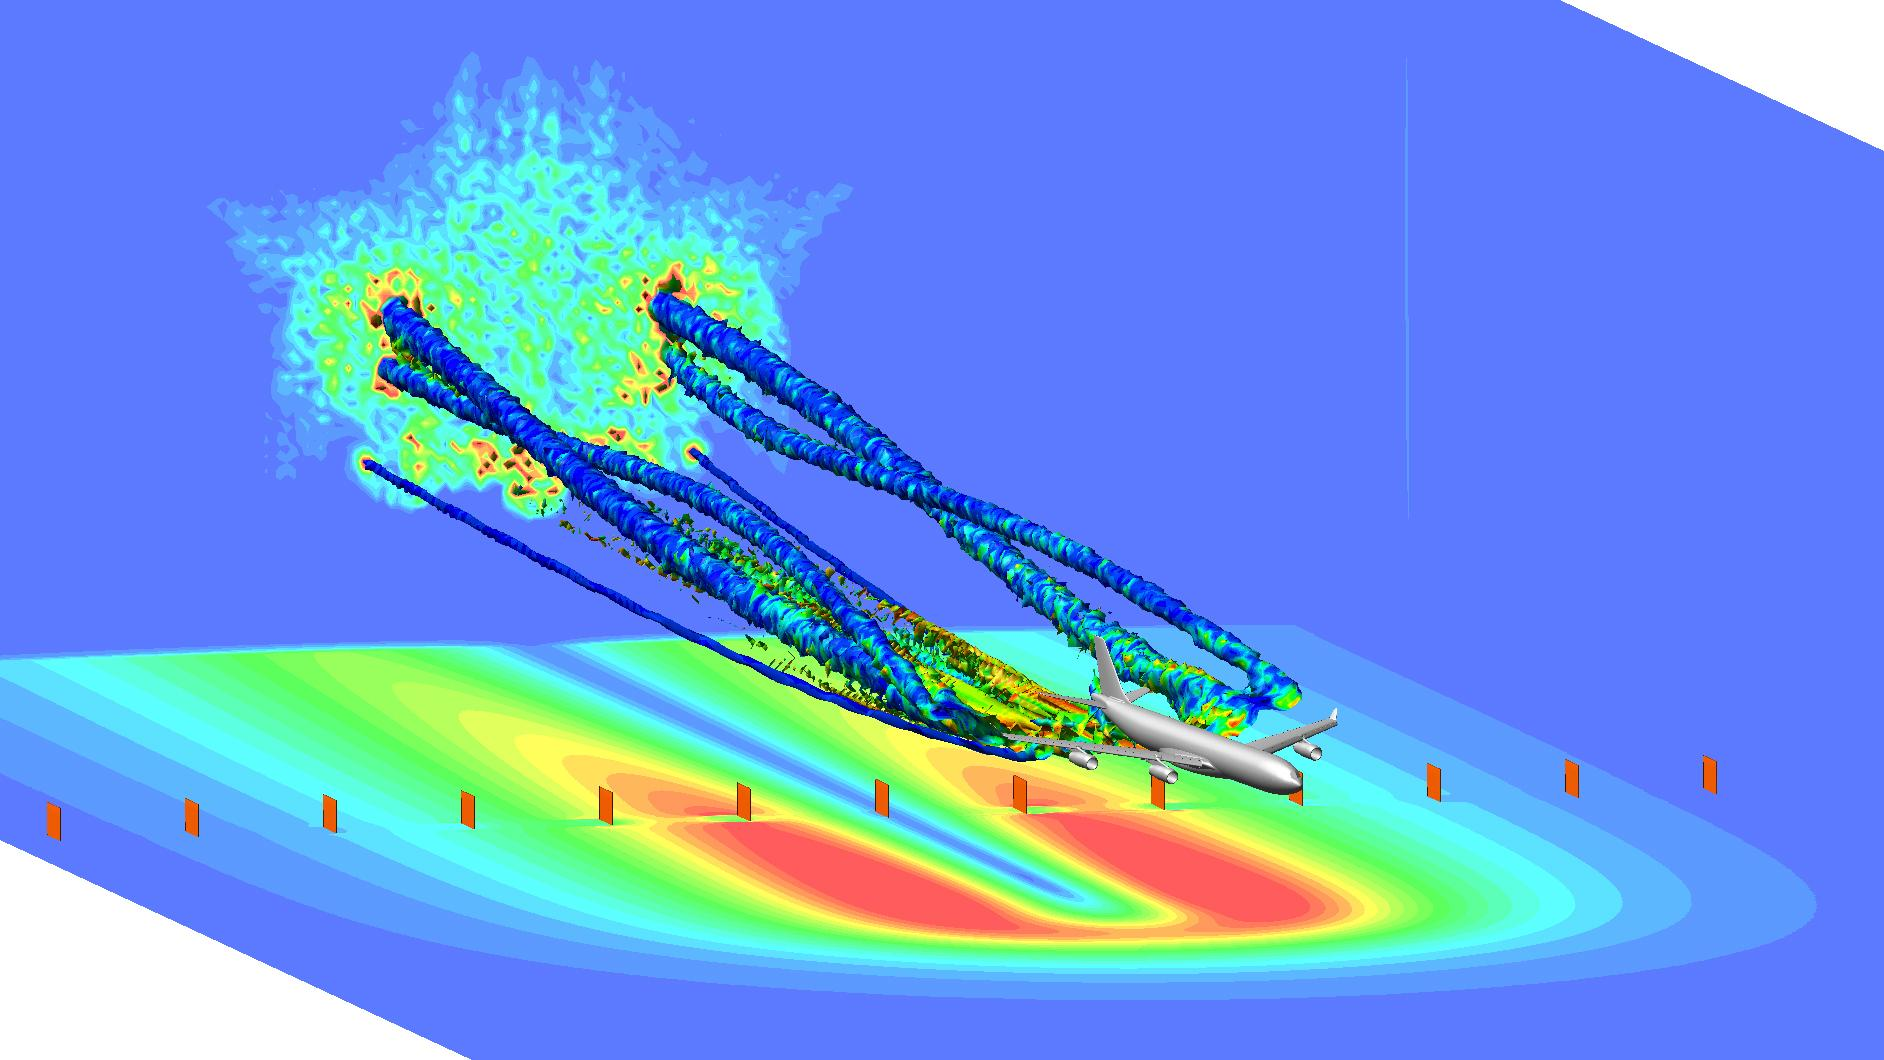
\includegraphics[width=0.8\textwidth]{papers/wirbelringe/fig/wirbelschleppen_in_der_simulation.jpg}
\caption{Simulation der Wirbelschleppenbildung eines Airbus A340 im Endanflug kurz vor der Landebahn
\cite{Wirbelringe:wirbelschleppen_in_der_simulation}. \label{Wirbelringe:fig:wirbelschleppen_in_der_simulation}}
\end{figure}

\subsection{Entstehung}
Wirbelschleppen bilden sich genau am Ende der Tragfläche aufgrund des Druckunterschieds, der das Flugzeug in erster Linie fliegen lässt.
Setzt sich ein Flugzeug in Bewegung, so entsteht um die Flügeltragflächen ein Luftstrom.
Ein weitverbreiteter Irrglaube besagt, dass die Luft, die über den Flügel geht, einen „längeren“ Weg zurücklegt und deshalb schneller sein muss, um sich am Ende wieder mit der Luft unter dem Flügel zu „treffen“.
Dies ist jedoch physikalisch nicht korrekt.
Die Luftströmung über dem Flügel wird nicht durch ein gleichzeitiges Eintreffen bestimmt, sondern durch die Geometrie des Flügels und die daraus resultierenden Strömungsverhältnisse.

Um diese Verhältnisse mathematisch zu beschreiben, betrachtet man zwei gedachte Stromröhren --- eine über und eine unter dem Flügel. 
Nach dem Prinzip der Massenerhaltung muss durch jede dieser Stromröhren dieselbe Luftmasse pro Zeit hindurchströmen. Dies führt zur Kontinuitätsgleichung
\begin{equation*}
v_{\text{oben}}A_{\text{oben}} 
=
v_{\text{unten}}A_{\text{unten}}.
\end{equation*}
Mithilfe derselben und dem Satz von Bernoulli
\begin{equation}
    p+\frac{1}{2}\rho v^2+\rho gh
    =
    \text{const}
    \label{Wirbelringe:eq:Bernoulli},
\end{equation}
kann jeweils ein Punkt auf der Oberseite sowie einer auf der Unterseite in \eqref{Wirbelringe:eq:Bernoulli} eingesetzt werden.
So können sie 
\begin{equation*}
p_{\text{oben}}+\frac{1}{2}\rho v^2_{\text{oben}} + \rho gh_1 
=
p_{\text{unten}}+\frac{1}{2}\rho v^2_{\text{unten}}+\rho gh_2
\end{equation*}
gleichgesetzt werden.
Jetzt kann angenommen werden, dass der Höhenunterschied zwischen den beiden Punkten oberhalb und unterhalb des Flügels vernachlässigbar klein ist, also \(h_1\approx h_2\).
Zudem ist die Dichte der Luft an beiden Punkten ungefähr gleich, weshalb sich der Term zu 
\begin{equation*}
p_{\text{oben}}+\frac{1}{2}\rho v^2_{\text{oben}} 
=
p_{\text{unten}}+\frac{1}{2}\rho v^2_{\text{unten}}
\end{equation*}
vereinfacht.
Für die Druckdifferenz ergibt sich
\begin{equation*}
p_{\text{oben}}-p_{\text{unten}} 
=
\frac{1}{2}\rho( v^2_{\text{unten}}-v^2_{\text{oben}})
\end{equation*}
und man kann erkennen, wenn \(v_{\text{unten}} < v_{\text{oben}}\) dann muss \(p_{\text{unten}} > p_{\text{oben}}\) sein.

Mit diesem Wissen kann auch die Entstehung der Wirbelschleppe erklärt werden. 
Es existiert also unterhalb des Flügels ein Überdruck und oberhalb ein Unterdruck.
Solange ein Flügel dazwischen ist, generiert dieser Druckunterschied einen Auftrieb, was gut und auch gewünscht ist.
Allerdings endet der Flügel an einer bestimmten Stelle und dort wird es interessant.
An der Spitze des Flügels findet nämlich ein Druckausgleich statt.
Hierbei strömt die Luft unterhalb des Flügels nach oben in den Bereich mit geringerem Druck. 
Die Luft zirkuliert dabei mit der Zirkulation \(\Gamma\) um das Flügelende und bildet eine ringförmige Strömung.
Schliesslich wird sie zu einer Wirbelschleppe am Flügelende.
Die entstandene Wirbelschleppe hat ein paar interessante Eigenschaften.

\subsection{Wirbellinie}
Wie bereits im Kapitel \ref{Wirbelringe:Wirbellinien} erwähnt sind Wirbellinien immer geschlossen oder enden auf Grenzflächen.
Die Wirbellinie der Wirbelschleppe startet am Flügelende (Grenzfläche zwischen Luft und Aluminium) und verläuft quer über die Startpiste.
Dort schliesst sie sich dann am anderen Flügelende wieder an der Grenzfläche zwischen Luft und Aluminium.
Landet das Flugzeug und kommt zum Stehen, löst sich die Wirbellinie von den Flügelenden ab und schliesst sich hinter dem Flugzeug.
Das bedeutet: In der Theorie entsteht ein „Wirbelring“, welcher quer über die Startpiste „parallel“ bis zum Zielflughafen und dann wieder quer über die Landebahn verläuft.
Dies klingt zunächst etwas seltsam und unglaubwürdig und natürlich ist diese Aussage auch nicht ganz korrekt.
In der Realität löst sich die Wirbelschleppe mit der Zeit durch Luftwiderstand auf und damit auch die zugehörigen Wirbellinien.
Also gibt es leider oder eben zum Glück keinen riesigen Wirbelring von Zürich nach Tokyo, wenn man mit dem Flugzeug etwaige Enkel besucht.

\begin{figure}
\centering
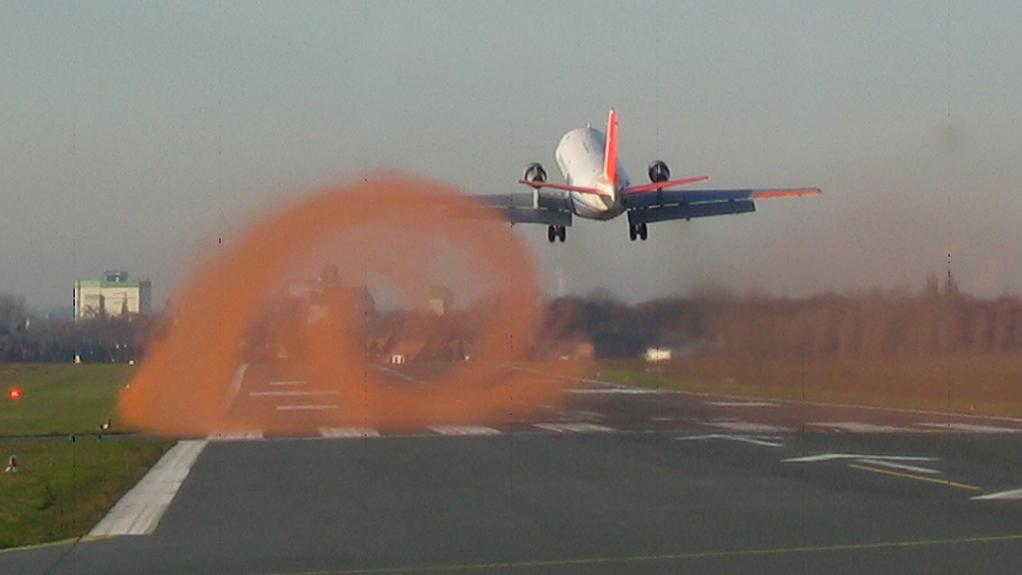
\includegraphics[width=0.8\textwidth]{papers/wirbelringe/fig/visualisierung_einer_wirbelschleppe.jpg}
\caption{Sichtbar gemachte Wirbelschleppe 
\cite{Wirbelringe:visualisierung_einer_wirbelschleppe} \label{buch:papers:Wirbelringe:fig:visualisierung_einer_wirbelschleppe}}
\end{figure}

\subsection{Problematik in der Aviatik}
Da Wirbelringe sehr stabil sind und sich nicht sofort auflösen, bleiben auch die Wirbelschleppen relativ lange bestehen.
Zudem breiten sie sich seitlich aus und sinken hinter dem Flugzeug ab.
Bei „schweren“ Flugzeugen (ab 136 Tonnen MCTOW\footnote{Maximum certified takeoff weight oder zu Deutsch: maximales Startgewicht}) ist vorgeschrieben \cite{Wirbelringe:WakeTurbulence}, dass nachfolgende Flugzeuge bis zu 3 Minuten warten müssen, bevor sie starten dürfen.
Denn, sollte ein Kleinflugzeug kurz nach einem solchen Flugzeug starten, wird es ziemlich sicher von dessen Wirbelschleppe erfasst.
In ganz schlimmen Fällen kann dies durchaus zu einem Absturz führen.

Ebenfalls muss man bedenken, dass es Energie benötigt, eine solche Wirbelschleppe aufrechtzuerhalten.
Die Energie dafür wird natürlich aus den Triebwerken des Fliegers gewonnen, die aber eigentlich dafür gedacht war, Passagiere von A nach B zu bringen.
Deshalb finden die Airlines es grundsätzlich nicht sehr amüsant, zwei gewaltige Wirbelschleppen hinter ihren Flugzeugen herzuziehen, auch wenn es bei schlechtem Wetter sehr spektakulär aussehen kann (siehe Abbildung \ref{Wirbelringe:fig:visualisierung_einer_wirbelschleppe}). 
Findige Wissenschaftler waren deshalb auf die Idee der Winglets gestossen.
Diese sollten durch Reduktion der Zirkulation an den Flügelenden die Bildung solcher Wirbelschleppen hemmen.
Bei diesem Unterfangen hatten sie auch Erfolg aber zu einem Preis, der in der Aviatik nicht gern gesehen ist.
Durch das Anbringen solcher Winglets an den Flügelenden steigt das Leergewicht des Flugzeuges an.
Das bedeutet, dass dieses zusätzliche Gewicht wieder mehr Treibstoff verbraucht.
Wieso werden diese aber trotzdem in Kurzstreckenflugzeugen eingesetzt?
Einerseits haben Winglets zusätzlich die angenehme Eigenschaft, den Lärm eines Flugzeuges zu reduzieren.
Andererseits höhlt bekanntlich steter Tropfen den Stein.
Wenn ein Kurzstreckenflieger täglich 5--6-mal fliegt und dabei jedes Mal 1--2 \% Treibstoff spart, so summiert sich dies und wird wieder lohnend für die Fluggesellschaften.
Bei Langstreckenflügen hingegen lohnen sich die Winglets noch viel mehr, da bei längerem Flug auf Reiseflughöhe (\textasciitilde10000 Meter über dem Meeresspiegel) auch die maximale Wirkung der Winglets länger genutzt werden kann.
